\chapter{Appendix B}
\label{chp:appendixb}

Appendix B contains screenshots and detailed figures from the measurements done in the network built in this thesis. This is meant to be a supplement to the figures presented earlier in the thesis to give the reader a deeper understanding of the system. In addition to the measurements presented here, all data gathered from the system and code used will be public GitHub, \url{http://github.com/sische/MasterThesis}. 

The following capture shows a part of a Wireshark capture, as described in chapter \ref{chp:measurements2}.1. This capture shows a \gls{payload} of 0 byte sent using \gls{coap} \gls{non}, and was the base for values used in table \ref{coapCON0table}. 

\begin{figure}[ht]
    \centering
    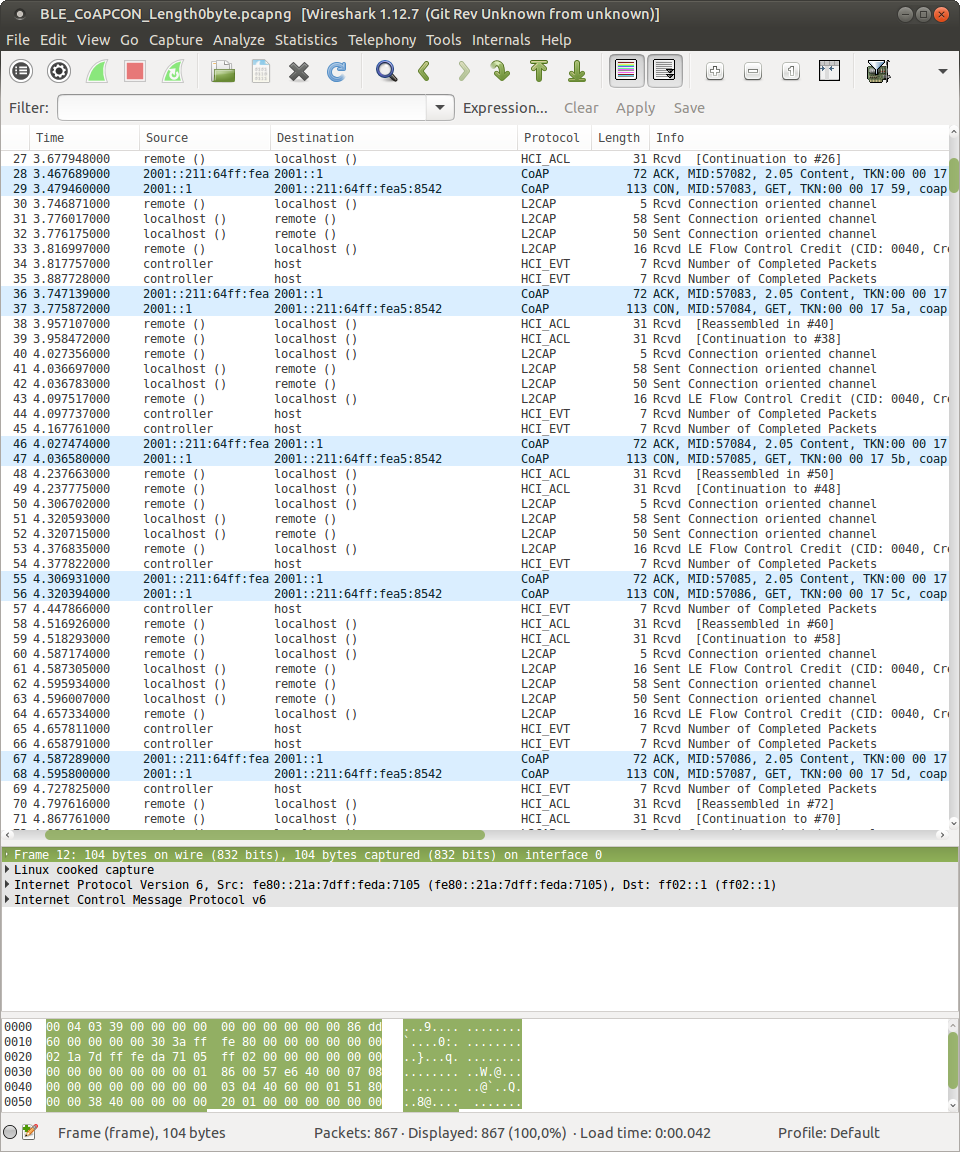
\includegraphics[width=1.1\textwidth]{0byteCONwireshark.png}    
    \caption{Wireshark capture, 0 bytes C. }
    \label{fig:wireshark0byteCONappendixB}
\end{figure}


%\begin{center}
% \begin{tabular}{||c c c c||} 
% \hline
% Goodput & Throughput & NON packet size & (Goodput/Throughput)*100 \\ [0.5ex] 
% \hline\hline
% 0 & 71 & 76 & 0 \\ 
% \hline
% 1 & 73 & 78 & 1,37 \\
% \hline
% 10 & 82 & 87 & 12,20 \\
% \hline
% 20 & 92 & 97 & 21,74 \\
%  \hline
% 30 & 75 & 107 & 30,0 \\
%  \hline
% 40 & 85 & 117 & 47,06 \\
%  \hline
% 50 & 99 & 127 & 50,51 \\
%  \hline
%60 & 109 & 137 & 55,05 \\
% \hline
% 70 & 119 & 147 & 58,82 \\
%  \hline
% 80 & 133 & 157 & 60,15 \\
%  \hline
% 90 & 143 & 167 & 62,94 \\
% \hline
% 100 & 153 & 177 & 65,36 \\
% \hline
% 110 & 167 & 187 & 65,87 \\
% \hline
% 120 & 177 & 197 & 67,80 \\
% \hline
% 130 & 191 & 207 & 68,06 \\
% \hline
% 140 & 207 & 217 & 69,65 \\
% \hline
% 150 & 211 & 227 & 71,09 \\
% \hline
% 160 & 225 & 237 & 71,11 \\
% \hline
% 170 & 235 & 247 & 72,34 \\
% \hline
% 180 & 253 & 257 & 71,15 \\
% \hline
% 190 & 263 & 267 & 72,24 \\
% \hline
% 200 & 277 & 277 & 72,20 \\ [1ex] 
% \hline
%\end{tabular}
%\caption{Measurements, BLE, constant length}
%\label{table:1}
%\end{center}